\documentclass[a4paper,oneside,12pt,titlepage]{scrartcl}   %Grundeinstellungen

\usepackage[ngerman]{babel}
%\usepackage[T1]{fontenc} % umlaute
\usepackage[utf8]{inputenc}
\usepackage{setspace}
\usepackage{amsfonts}
\usepackage{amsmath}
\usepackage{amssymb}
\usepackage{amsthm}
\usepackage{subfiles} 
\usepackage{caption}
\usepackage{hyperref}
\usepackage{ragged2e}
\usepackage{wrapfig}
\usepackage[amssymb]{SIunits}
\usepackage{cite}
\usepackage[usenames,dvipsnames]{xcolor}
\usepackage{listings}
\usepackage{textcomp}

\definecolor{comment}{RGB}{0,128,0} % dark green
\definecolor{string}{RGB}{255,0,0}  % red
\definecolor{keyword}{RGB}{0,0,255} % blue

\lstdefinestyle{c}{
	commentstyle=\color{comment},
	stringstyle=\color{string},
	keywordstyle=\color{keyword},
	basicstyle=\footnotesize\ttfamily,
	numbers=left,
	numberstyle=\tiny,
	numbersep=5pt,
	frame=lines,
	breaklines=true,
	prebreak=\raisebox{0ex}[0ex][0ex]{\ensuremath{\hookleftarrow}},
	showstringspaces=false,
	upquote=true,
	tabsize=2,
}
 \lstset{language=c} 


\renewcommand{\familydefault}{\sfdefault} 
\usepackage{graphicx}
\usepackage{subcaption}                       
\usepackage{float}
\usepackage[section]{placeins}
\renewcommand{\topfraction}{0.85}
\renewcommand{\textfraction}{0.1}
\renewcommand{\floatpagefraction}{0.75}

\usepackage{cite}
\usepackage[usenames,dvipsnames]{xcolor}


\usepackage{listings}

\lstset{%
	 basicstyle=\scriptsize\ttfamily,
   keywordstyle=\bfseries\ttfamily\color{NavyBlue},
   stringstyle=\color{Rhodamine}\ttfamily,
   commentstyle=\color{Green}\ttfamily,
   emph={square}, 
   emphstyle=\color{blue}\texttt,
   emph={[2]root,base},
   emphstyle={[2]\color{yac}\texttt},
   language=Python,%
   tabsize=2,%
   basicstyle=\footnotesize\ttfamily,%
   numbers=left,%
   numberfirstline,%
   breaklines=true,%
   breakatwhitespace=true,%
   linewidth=\textwidth,%
   xleftmargin=0.075\textwidth,%
   frame=tlrb,%
   captionpos=b%
}


%Header Definitionen
\usepackage{fancyhdr}
\renewcommand{\headrulewidth}{0.5pt}
\renewcommand{\footrulewidth}{0.5pt}
%Abstand zwischen Absätzen, Zeilenabstände
\voffset26pt 
\parskip6pt
%\parindent1cm  %Rückt erste Zeile eines neuen Absatzes ein
\usepackage{setspace}
\onehalfspacing

\begin{document}
\pagenumbering{arabic}

% Titeseite
\begin{titlepage}
\begin{center}
	\begin{minipage}{0.6\textwidth}
	\begin{tabular}{l}
	Technische Universität Berlin\\
	Fakulät IV (Elektrotechnik und Informatik)\\
	Institut für Energie- und Automatisierungstechnik\\
	Fachgebiet Lichttechnik\\
	\end{tabular}
	\end{minipage}
	\hfill
	\begin{minipage}{0.3\textwidth}\raggedright
	
\includegraphics[scale=0.06]{tu-logo}\\
	\end{minipage}
	
	\vspace{3cm}
    \sffamily \LARGE \textbf{Entwicklung und Realisierung einer Messeinrichtung mit den Sensoren AS7261 und AS72651 von ams}\\
 	\Large Bachelorarbeit\\
    \vspace{2.5cm}
	{\renewcommand{\arraystretch}{0.7}
    	\begin{tabular}{ll}
    		Vorgelegt von: & Lennard Bödiger\\
			Studiengang:	 & Technische Informatik\\
			Matrikel-Nr.: & 363470\\
		\end{tabular}
	}

  	\vspace{5.3cm}
	\end{center}
	\begin{tabular}{ll}
		Eingereicht am: & 8. Februar 2021\\
		Betreuung: & Nils Weber\\
		Prüfer/in: & Prof. Dr.-Ing. Stephan Völker Prof.\\ 	& Dr.-Ing. Sibylle Dieckerhoff
	\end{tabular}\\
\end{titlepage}
\newpage
\begin{figure}[H]
\centering
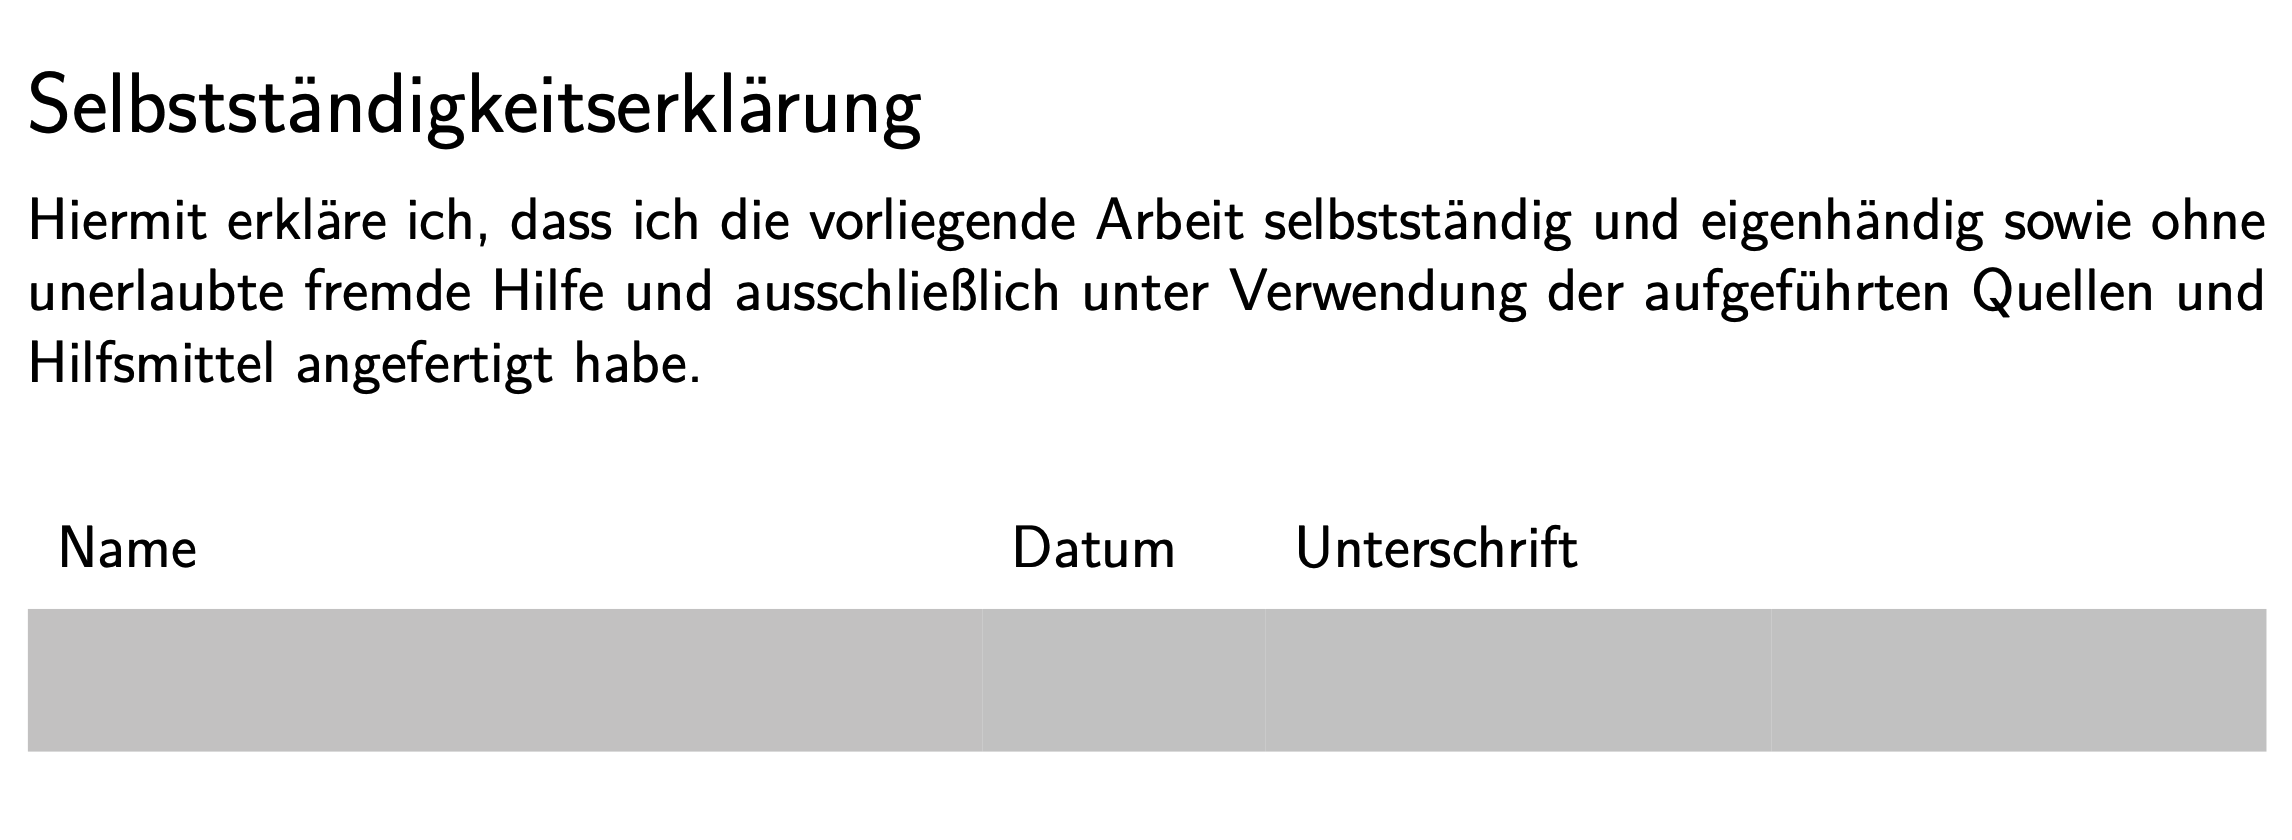
\includegraphics[width=1\textwidth]{img/alles-ich.png}
\end{figure}

\newpage

\section*{Abstract}
\subfile{sections/Abstract}
\newpage
\tableofcontents
\newpage
\listoffigures
\newpage
\listoftables
\section{TODO Liste}
anhangsverzeichniss\\
der satz von dem foto ist müll\\


\newpage
\section{Einleitung}
\subfile{sections/Einleitung}
\newpage
\section{Technische Grundlagen}
\subfile{sections/Technische_Grundlagen}
\newpage
\section{Hardware Komponenten}
\subfile{sections/Hardware_Komponenten}
\newpage
\section{Platine}
\subfile{sections/Platine}
\newpage
\section{Datenbank \& Webinterface}
\subfile{sections/Datenbank_und_Webinterface}
\newpage
\section{C Code}
\subfile{sections/Software}
\newpage
\section{Benutzerhandbuch}
\subfile{sections/Benutzerhandbuch}
\newpage
\section{Messungen}
\subfile{sections/Messungen}
\newpage
\section{Zusammenfassung}
Der Raspberry Pi hat sich als Steuergerät für den Messaufbau bewährt.
Programmcode kann schnell und einfach über SSH ausgeführt werden und auch die Fehlersuche ist sehr komfortabel.\\
Grafana lässt sich in der grafischen Oberfläche sehr einfach anpassen, aber das einmalige Einrichten eines Dashboards ist für viele Sensoren umständlich und zeitaufwendig.
Die Datenkomprimierungseffizienz von InfluxDB übertrifft die Erwartungen, sodass es möglich ist, auch mit kleinen SD-Karten über mehrere Jahre Daten zu erfassen.\\
Alle Softwarekomponenten laufen im Dauertest mit einer angeschlossenen Sensorplatine seit sechs Wochen ohne Probleme.
In einem weiteren Test läuft das System mit 4 angeschlossenen Sensorboards seit zwei Wochen ebenfalls ohne Probleme.\smallskip

\noindent Zum Abgabezeitpunkt der vorliegenden Arbeit besteht das Problem, dass nur vier Sensorplatinen d.h. 8 I2C-Salven gleichzeitig am Bus angeschlossen werden können.
Ab dem fünften Sensorboard kann der Raspberry Pi die I2C-Adressen aller angeschlossenen Sensoren nicht mehr finden.
Das Problem könnte mit einem modernen Oszilloskop analysiert werden, aber die Verfügbarkeit von Werkzeugen ist aufgrund der Corona-Pandemie zeitnah nicht möglich.
Als Workaround gibt es die Möglichkeit, einen Bus-Multiplexer zu verwenden.
Dieses Gerät wird über i2c direkt an den Bus angeschlossen und hat mehrere I2C-Bus-Ports, über einen Befehl kann dem Multiplexer mitgeteilt werden, welcher I2C-Bus-Kanal zum Raspberry Pi durchgeschaltet wird.
Eine Betaversion des Workarounds ist bereits implementiert und auf Github\footnote{\url{https://github.com/LennardBoediger/Bachelorarbeit}} zu finden, wird aber in dieser Arbeit nicht behandelt.
\smallskip

\noindent Abgesehen davon, dass die geforderte Anzahl der anschließbaren Sensoren derzeit nicht erreicht wird, ist der Messaufbau einsatzbereit und die verbleibenden Probleme können mit überschaubarem Aufwand gelöst werden.
\newpage
\bibliography{Quellen/Quellen.bib}
\bibliographystyle {ieeetr}
\end{document}